\documentclass[12pt]{article}
\usepackage[a4paper, total={7.5in, 10in}]{geometry}
\usepackage{array}
\usepackage{graphicx, subfig, wrapfig, fancyhdr, lastpage, multicol ,color,arydshln,makecell, chemfig}

\newcommand\headerMe[2]{\noindent{}#1\hfill#2}
\usepackage[mathscr]{euscript}
\usepackage{tabularray}

\setlength{\columnseprule}{1pt}
\def\columnseprulecolor{\color{blue}}


\pagestyle{fancy}
\fancyhf{}

\cfoot{ \em{Page \thepage \hspace{1pt} / \pageref{LastPage}}}
\begin{document}

\headerMe{Royaume du Maroc}{année scolaire \emph{2023-2024}}\\
\headerMe{Ministère de l'Éducation nationale, }{  Professeur :\emph{Zakaria Haouzan}}\\
\headerMe{du Préscolaire et des Sports}{Établissement : \emph{Lycée SKHOR qualifiant}}\\
%\vspace{-1cm}
\begin{center}
Devoir Surveillé  N°2 - S2 \\
    2ème année baccalauréat Sciences physiques\\
Durée 2h00
\\
    \vspace{.2cm}
\hrulefill
\Large{Chimie 7pts - 45min}
\hrulefill\\

    %\emph{Les deux parties sont indépendantes}
\end{center}
%end Headerss------------------------
%__________________Chimie ______________________-
%%%%%%%+_+_+_+_+_+_+_+_+_Partie1

 \section*{Partie I- Electrolyse d’un composé ionique : le bromure de plomb}
%\begin{wrapfigure}{r}{0.16\textwidth}
	%\vspace{-1.2cm}
%%\begin{center}
  %%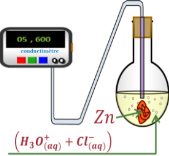
\includegraphics[width=0.16\textwidth]{./img/chimie01.png}
%%\end{center}
%\end{wrapfigure}

On réalise l’électrolyse du bromure de plomb $Pb^{2+} + 2Br^- $ à haute température par un générateur
fournissant un courant électrique d’intensité I constante.
Au cours de cette électrolyse, le métal plomb se dépose sur l’une des électrodes et au niveau de
l’autre, il se forme le gaz dibrome.
Au cours du fonctionnement de l’électrolyseur pendant la durée $\Delta{t} =3600s$, la masse de plomb
déposé est : $m = 20,72g$.


\textbf{\underline{Données:}}
\begin{itemize}
  \item Les 2 couples mis en jeu : $Pb^{2+}/Pb_{(s)}$ et $Br_{2(g)}/Br^-$
  \item La constante de Faraday : $F=9,65.10^{4} C.mol^{-1} $;
  \item Le volume molaire des gaz dans les conditions de l’expérience $V_m = 70,51L/mol$
  \item La masse molaire du plomb: $M(Pb) = 207,2 g/mol $.
\end{itemize}

\begin{enumerate}
  \item Donner le nom de l’électrode (anode ou cathode) au niveau de laquelle se forme le dibrome\dots(0,5pt)
  \item Ecrire les équations des réactions aux électrodes, ainsi que l’équation bilan lors de
    l’électrolyse\dots(1pt)
\item Déterminer la valeur de l’intensité I du courant électrique passant dans le circuit pendant la
  durée $\Delta{t}$\dots(1pt)
\item Calculer, dans les conditions de l’expérience, le volume V du gaz dibrome formé pendant $\Delta{t}$\dots(1pt)
\end{enumerate}


 \section*{Partie II- Etude de la pile zinc-cuivre}
\emph{Lors de leur fonctionnement, les piles électrochimiques convertissent une partie de l’énergie
chimique en énergie électrique. On étudie dans cette partie de l’exercice le principe de
fonctionnement de la pile zinc-cuivre.}

On réalise la pile zinc-cuivre en utilisant le matériel et les produits suivants :
\begin{itemize}
  \item un bécher contenant une solution aqueuse de sulfate de zinc $Zn^{2+}_{(aq)} + SO^{2-}_{4(aq)}$ de concentration
molaire $C_1 =1 mol/L$

\item un bécher contenant une solution aqueuse de sulfate de cuivre $Cu^{2+}_{(aq)} + SO^{2-}_{4(aq)}$ de concentration
molaire $C_2 = 1mol/L$
\item une lame de zinc et une lame de cuivre.
\item un pont salin.
\end{itemize}
On relie les électrodes de la pile à un conducteur ohmique en série avec un ampèremètre qui
indique le passage d’un courant électrique d’intensité constante $I_A = 0,3$ dans le circuit.
\textbf{\underline{Données:}}
\begin{itemize}
  \item La constante de Faraday : $F=9,65.10^{4} C.mol^{-1} $.
  \item La masse molaire du cuivre: $M(Cu) = 63,5 g/mol$.
  \item La constante d'équilibre associée à l'équation $Cu^{2+}_{(aq)} + Zn_{(s)} \rightleftharpoons	
 Zn^{2+}_{(aq)} + Cu_{(s)} $ est $K =1,7.10^{37}$.
\end{itemize}


\begin{enumerate}
  \item Calculer la valeur du quotient de réaction $Q_{r,i}$ à l’état initial du système chimique.\dots(0,5pt)
  \item  En déduire le sens d'évolution spontanée du système chimique.\dots(1pt)
  \item Ecrire l’équation de la réaction chimique à la cathode.\dots(1pt)
  \item La pile fonctionne pendant une durée $\Delta{t} = 5h$ . Calculer la masse $m(Cu)$ Cu du cuivre déposé
    pendant la durée $\Delta{t}$.\dots(1pt)
\end{enumerate}

%\hrulefill
%\Large{Physique 13pts/78min}
%\hrulefill\\
%\newpage
\begin{center}
    %\vspace{.60cm}
\hrulefill
\Large{Physique 13pts - 75min}
\hrulefill\\
    \emph{Les  parties sont indépendantes}
\end{center}

%\vspace{-1cm}
\section*{Partie I : Etude de la chute d’une balle}
\begin{wrapfigure}[4]{r}{0.2\textwidth}
\begin{center}
  \vspace{-3cm}
  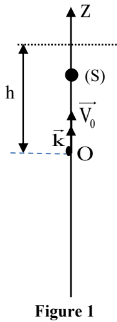
\includegraphics[width=0.12\textwidth]{./img/figP00.png}
\end{center}
\end{wrapfigure}


Dans le champ de pesanteur, on lance verticalement vers le haut à l’instant $t = 0$ à partir d’un point O,
une balle (S) de masse m et de centre d’inertie G , avec une vitesse initiale de valeur $V_0 = 12 m/s$

On étudie le mouvement du centre d’inertie G de la balle dans un repère $(O, \vec{k})$ lié à un
référentiel terrestre supposé galiléen en deux phases:

\begin{itemize}
  \item mouvement de chute libre de la balle dans la première phase.
  \item mouvement de chute de la balle avec frottement dans la deuxième phase.
\end{itemize}

\textbf{Données : }La masse $m = 80g$ ; L’intensité de la pesanteur $g = 10 m/s^2$

\textbf{Partie I : Mouvement de la balle en chute libre}
Pendant son mouvement le centre d’inertie G de la balle est considéré en chute libre.

\begin{enumerate}
  \item[1-1.] En appliquant la deuxième loi de Newton, déterminer les équations horaires
   numériques donnant la vitesse $v_z(t)$ et la position $z(t)$ du centre d'inertie G de la balle\dots(0,75pt)

  \item[1-2.] En utilisant les équations $v_z(t)$ et $z(t)$ déterminer :
    \begin{enumerate}
      \item la hauteur maximale h atteinte par G\dots(0,5 pt)
      \item la valeur algébrique $v_{OZ}$ de la vitesse de G lors de son passage vers le bas par le point O\dots(0,5 pt)
    \end{enumerate}
\end{enumerate}

\textbf{Partie II : Mouvement de chute de la balle avec frottement}
A partir de l’instant du passage du centre d’inertie G par le point O vers le bas, qu’on prend comme
nouvelle origine des dates $t = 0$, la balle est soumise, en plus de son poids $\vec{P}$ , à une force de frottement fluide modélisée par $\vec{P} = -\lambda.\vec{v}$ avec $\vec{v} = v_z.\vec{k}$ et $\lambda = 0,12SI$ (On néglige la poussée d’Archimède devant ces deux forces).
\begin{enumerate}
  \item Montrer que l’équation différentielle vérifiée par la vitesse $v_z$ du centre d’inertie G de la balle s’écrit : $\frac{dv_z}{dt} + \frac{1}{\tau}v_z + g = 0$ avec $\tau$ le temps caractéristique du mouvement\dots(0,5pt)
  \item Déduire la norme de la vitesse limite du mouvement du centre d’inertie G de la balle\dots(0,25pt)
  \item Déterminer, en utilisant la méthode d’Euler, la valeur algébrique $v_z(t_i)$ de la vitesse à l’instant $t_i$ sachant que l’accélération du mouvement à l’instant $t_{i - 1}$ est $a_{i-1} = 5m.s^{-2}$ et on prend le pas de calcul $\Delta{t} = 66ms$\dots(0,75pt)
\end{enumerate}

\section*{Partie 2 : Etude du mouvement d’un ballon dans un champ de pesanteur uniforme }
  Lors d’un service, un joueur de volley-ball, se trouvant à une distance D du
filet, frappe le ballon à une hauteur h du sol et lui communique une vitesse $\vec{V_0}$
faisant un angle $\alpha$ par rapport à l’horizontale.

   A cet instant choisi comme origine des dates $t_0 = 0$
, le centre d’inertie G du ballon est au point A (figure 1).
  
   \begin{center}
%	  \vspace{-2cm}
	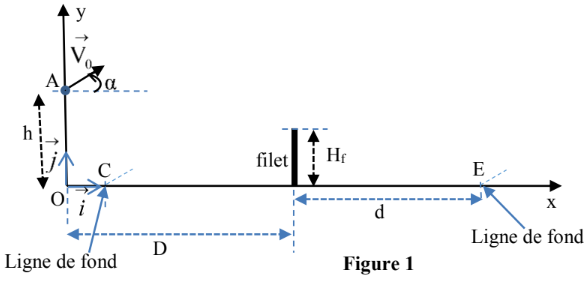
\includegraphics[width=0.6\textwidth]{./img/chute_libreSx.png}
  \end{center}
   \textbf{Données}

 \begin{itemize}
   \item $V_0 = 16 m/s$ ; $\alpha = 18^{\circ}$ ; $D=11m$ ; $h = OA= 3m$
   \item Hauteur du filet : $H_f = 2,4m$
   \item Distance entre le filet et la ligne de fond : $d =9m$
   \item Intensité de la pesanteur $g = 10 m.s^{-2}$
 \end{itemize}
   On étudie le mouvement du centre d’inertie G du ballon dans le repère $(O,\vec{i} , \vec{j} )$lié à un référentiel terrestre
considéré galiléen. L’origine O est situé au niveau du sol (figure 1).

On considère que le ballon est en chute libre.

\begin{enumerate}
  \item En appliquant la deuxième loi de Newton, établir les équations horaires x(t) et y(t) du mouvement de G. (1pt)
  \item Déduire que l’équation de la trajectoire du mouvement de G s’écrit: $$y = - \frac{1}{2}. \frac{g}{(V_0.cos\alpha)^2}.x^2 + (tan\alpha).x + h$$
  \item Montrer que le ballon passe au-dessus du filet (on néglige le rayon du ballon devant Hf). (0,75pt)
  \item Le ballon atteindra le sol à l’instant $t_s=1,41s$
    Le ballon tombe-t-il entre le filet et la ligne du fond du camp adverse? Justifier. (0,75pt)
\end{enumerate}

\section*{Exercice 1–un parcours de golf\dotfill(6pts)}

%\begin{wrapfigure}[9]{r}{0.25\textwidth}
  %\begin{center}
	  %\vspace{-1cm}
	%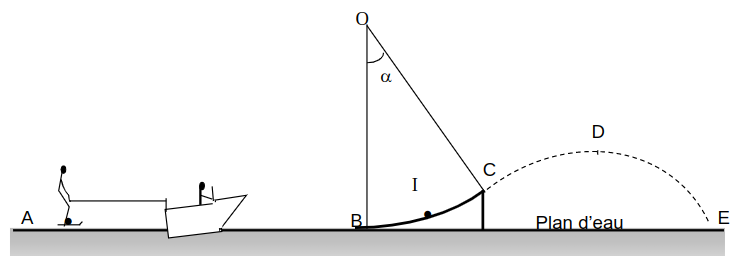
\includegraphics[width=0.19\textwidth]{./img/img01.png}
	%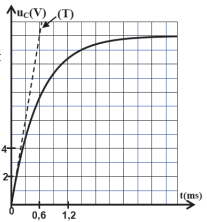
\includegraphics[width=0.25\textwidth]{./img/img02.png}
  %\end{center}
%\end{wrapfigure}

   % \begin{wrapfigure}[7]{r}{0.32\textwidth}
  %\begin{center}

	  %\vspace{-1.6cm}
	%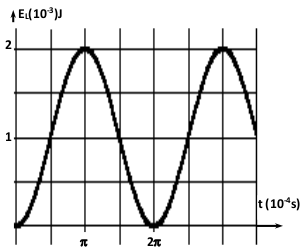
\includegraphics[width=0.32\textwidth]{./img/ex_02.png}
  %\end{center}
%\end{wrapfigure}

La figure ci-dessous schématise un parcours de golf. Le joueur désire envoyer la balle dans le trou
(drapeau) situé derrière un arbre d’une hauteur de $12 m$.

Le joueur, communique à la balle une vitesse initiale $V_0$ dont la direction du vecteur fait un angle $\alpha$
avec l’horizontale passant par l’origine de lancement. (figure 3 ci dessous) .

On suppose que les forces exercées par l'air sur la balle sont négligeables.



 \begin{center}
	  %\vspace{-1cm}
	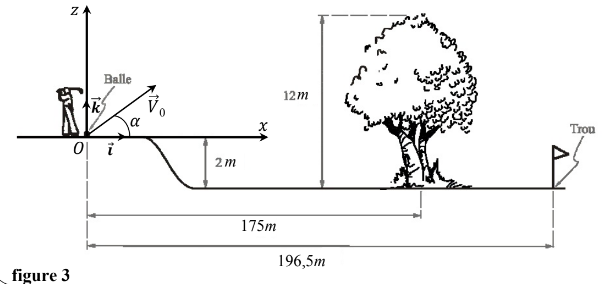
\includegraphics[width=0.8\textwidth]{./img/chute00.png}
  \end{center}


On étudie le mouvement de la balle dans le champ de pesanteur uniforme dans un repère orthonormé
$(O,\vec{i} , \vec{k})$ lié à la Terre considéré galiléen.

\begin{tabular}{c|l}	
	1 & \makecell[l]{\textbf{1. }En appliquant la deuxième loi de newton, déterminer les équations différentielles vérifiées \\par les
coordonnées $V_x$ et $V_z$ du vecteur vitesse de la balle dans le repère $(O, \vec{i} , \vec{k})$.}\\
	1 & \makecell[l]{\textbf{2. }Établir les équations horaires du mouvement $x(t)$ et $z(t)$. }\\
	0,75 & \makecell[l]{\textbf{3. }Vérifier que l’équation de la trajectoire s’exprime:$z = \frac{-g}{2.V_0^2.cos^2\alpha}.x^2 + xtan\alpha$ }\\
	0,75 & \makecell[l]{\textbf{4. }Les courbes de la figure 4 représentent les variations de $V_x$
et $V_z$
en fonction du temps\\ Vérifier que  : $v_0 \approx 46,04 m.s^{-1}$ et que $\alpha \approx 32,86^{\circ}$}\\
	1 & \makecell[l]{\textbf{5. }En déduire la valeur de g l’intensité de la pesanteur. }\\
	0,75 & \makecell[l]{\textbf{6. }Montrer que la balle passe au dessus de l’arbre. }\\
	0,75 & \makecell[l]{\textbf{7. }Est ce que le joueur a réalisé son objectif ?. }\\
\end{tabular}


 \begin{center}
	  %\vspace{-1cm}
	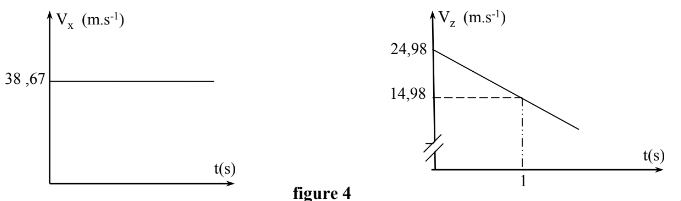
\includegraphics[width=0.8\textwidth]{./img/chute__01.png}
  \end{center}




%\begin{wrapfigure}[9]{r}{0.25\textwidth}
  %\begin{center}
	  %\vspace{-1cm}
	%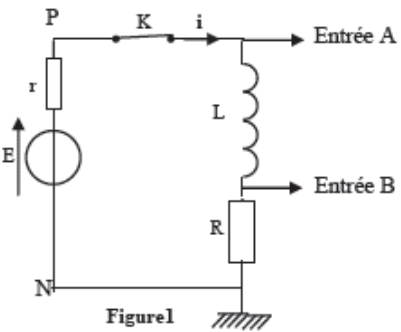
\includegraphics[width=0.22\textwidth]{./img/img03.png}
	%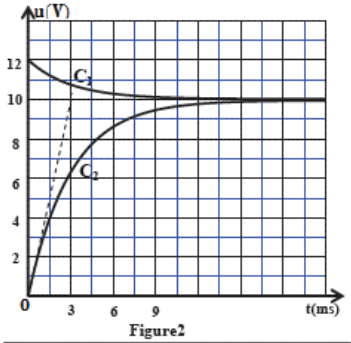
\includegraphics[width=0.25\textwidth]{./img/img04.png}
  %\end{center}
%\end{wrapfigure}



	%\vspace{0.5cm}
%\textbf{2. Injection locale d’une solution contenant du rhénium 186.
%Le produit injectable se présente sous la forme d’une solution contenue dans un flacon de volume $V_0= 10 mL$ ayant une activité $a_0 = 4.10^9Bq$ à la date $t=0$, c'est-à-dire à la sortie du laboratoire pharmaceutique.}
	%\begin{tabular}{c|l}

		%1 & \makecell[l]{\textbf{2.1 }Déterminer en jours la valeur de demi-vie $t_{1/2}$ du rhénium $_{75}^{186}Re$}\\

		%0,5 & \makecell[l]{\textbf{2.2 }Trouver, à l’instant $t_1 = 4,8jours$, le nombre $N_1$ de noyau de rhénium contenu dans le flacon.}\\

		%0,5 & \makecell[l]{\textbf{3.2 } À l’instant $t_1$ on prélève du flacon de volume $V_0 = 10mL$ une injection de volume V contenant \\$N = 3,65.10^{13}$ noyaux de rhénium 186, on l’injecte à un malade dans l’articulation de l’épaule, \\trouver la valeur de V.}\\
	%\end{tabular}


%\section*{Partie 2 :  Centrale nucléaire \dotfill(9pts)}
%Dans une centrale nucléaire, les noyaux d'uranium $^{235}_{92}U$ subissent la fission sous le choc d'un neutron
%lent. Un des nombreux processus possibles conduit à la formation d'un noyau de lanthane $^{144}_{57}La$ ,d'un noyau de brome $^{88}_{35}Br$ et  de plusieurs neutrons.

%\begin{tabular}{c|l}

 %1& \makecell[l]{\textbf{1. } Définissez l'énergie de liaison d'un noyau.}\\

 %1 & \makecell[l]{\textbf{2. } Donnez l'expression littérale qui permettra son calcul.}\\

 %1 & \makecell[l]{\textbf{3. } Calculez, en MeV, l'énergie de liaison d’un noyau $^{235}_{92}U$.}\\

 %1 & \makecell[l]{\textbf{4. } Calculez l’énergie de liaison par nucléon de ce noyau.}\\

 %1 & \makecell[l]{\textbf{5. } Ecrivez l’équation de la réaction de fission étudiée.}\\

 %1 & \makecell[l]{\textbf{6. } Exprimez l'énergie libérée par la fission d'un noyau $^{235}_{92}U$ en fonction des énergies de liaison par
%\\ nucléon du noyau père et des noyaux fils et calculez la valeur de cette énergie en MeV.}

 %\end{tabular}

%\textbf{7.  Dans le cœur de la centrale, de nombreuses autres réactions de fission du noyau $^{235}_{92}U$ se produisent. La perte de masse est, en moyenne, de 0,200 u par noyau.}


%\begin{tabular}{c|l}

	%1,5 & \makecell[l]{\textbf{7.1. } Calculez, en MeV, l'énergie moyenne libérée par la fission d’un noyau. Ce résultat est-il \\en concordance avec celui de la question 6 ?}\\

	%1,5 &\makecell[l]{\textbf{7.2. }Calculez, en joule, l'énergie moyenne libérée par une mole de noyaux $^{235}_{92}U$ } 

%\end{tabular}

%\textbf{Données :}
%\begin{itemize}
	%\item Célérité de la lumière dans le vide : $c = 2,998 . 10^8 m.s^{-1}$  
	%\item Masse du noyau d’uranium 235 : $m( ^{235}_{92}U) = 235,0134u$ 

	%\item Energies de liaison par nucléon : $E_l/A(^{144}_{57}La) = 8,28MeV/nucl$éon  ; $E_l/A(^{88}_{35}Br)$=$8,56MeV/nucl$éon
	%\item Constante d'Avogadro : $N_A = 6,02.10^{23} mol^{-1}$
	%\item $1u$ = $1,66055.10^{-27}Kg$ et $1eV = 1,602.10^{-19}J$
	%\item Masse d’un proton : $m(^1_1p) = 1,0073u$ ; Masse d’un neutron $m(^1_0n) = 1,0087u$
%\end{itemize}





\end{document}
